\section{目的}

依講義 PDF 第 115--118 頁比較完整與簡化單相 latch、double N/P clocked inverter，以及完整/縮減第一級的兩級 DFF 鏈。另加資料於相位中途改變的測試，驗證題目所問限制。

\section{講義要求與對應測試}

\begin{center}
\small
\setlength{\tabcolsep}{4pt}
\begin{tabular}{p{.42\linewidth}p{.29\linewidth}p{.18\linewidth}}
\toprule
要求 & 網表編號與條件 & 狀態 \\
\midrule
步驟 1：圖 28.1 a/c、b/d 比較 & 01; independent copies & 波形與差異已量測 \\
步驟 2：double N/P inverter 保持 & 02; data changes while held & 保持窗已量測 \\
問題 1：P/N latch 組 DFF 串兩級 & 03; 0.2/1 ns clock edges & 規律資料已量測 \\
問題 2：去除第一級、限制與內部點 & 03/04; periodic and hazard data & 反例已保留 \\
\bottomrule
\end{tabular}
\end{center}

\section{拓樸與預期行為}

圖 28.1(a)/(b) 的第二級為完整 clocked inverter；(c)/(d) 移除在相應動態節點狀態下多餘的互補 clock 元件。完整 DFF 由 P section 再接 N section，共四個反相級；縮減版去掉第一級後為三個反相級，單級輸出極性相反。串兩級時需按各自的反相數建立預期值，不能直接把第一級輸出波形逐點相減。

單相架構省去外部兩相時脈，但不代表每個內部節點都成為靜態記憶。動態預充/評估節點可能只允許一個方向的轉換；完整結構與縮減結構對輸入在相位內的變動容忍也不相同。

\section{模擬設定與判讀方式}

以提供的加密 MOS 模型、1.0 V 供應、25\,$^\circ$C 為基準。1.0 V 是教學測試條件，並非已核實的額定電壓；沒有把本次結果當作講義原製程或原供應電壓的重現。除網表另註，$W_n/W_p/L=0.6/1.8/0.25\,\mu\mathrm m$，Bulk 接對應電源軌，輸出負載為 5 fF。傳輸閘與弱回授器件的例外尺寸均在網表明列。

使用 PrimeSim HSPICE S-2021.09 win64、\texttt{RUNLVL=6}、\texttt{ACCURATE} 及 \texttt{WARNLIMIT=100}。每份網表的主分析與 \texttt{.alter} 均完成，沒有 error 或 failed measurement；但模擬器仍回報加密區塊的警告被隱藏，因此不能宣稱模型無警告或警告無害。\texttt{.tran} 的列印間隔不是固定積分步長；求解器使用自適應步長。本次沒有把有限的掃描範圍當作完整製程認證。

除非另註，功能診斷以低電位 $V\leq0.2$ V、高電位 $V\geq0.8$ V 判定；這是本報告公開採用的判讀規則，不是講義給定的數值門檻，也不是已萃取的接收器雜訊容限。取樣正確不能排除取樣間毛刺。所有圖均由實際輸出資料重繪；\texttt{results/} 保存逐案例波形、量測與衍生比較 CSV。

公開網表不含模型載入路徑；模擬時在本機副本加入模型設定，模型本體不在交付資料內。網表檔名的前兩位數對應下表編號，各檔可獨立執行。

\section{結果}

\begin{center}
\small
\setlength{\tabcolsep}{4pt}
\begin{tabular}{lr}
\toprule
配對 & 最大取樣電位差 (V) \\
\midrule
1-3 & 0.174150 \\
2-4 & 0.043550 \\
\bottomrule
\end{tabular}
\end{center}

\begin{figure}[htbp]
\centering
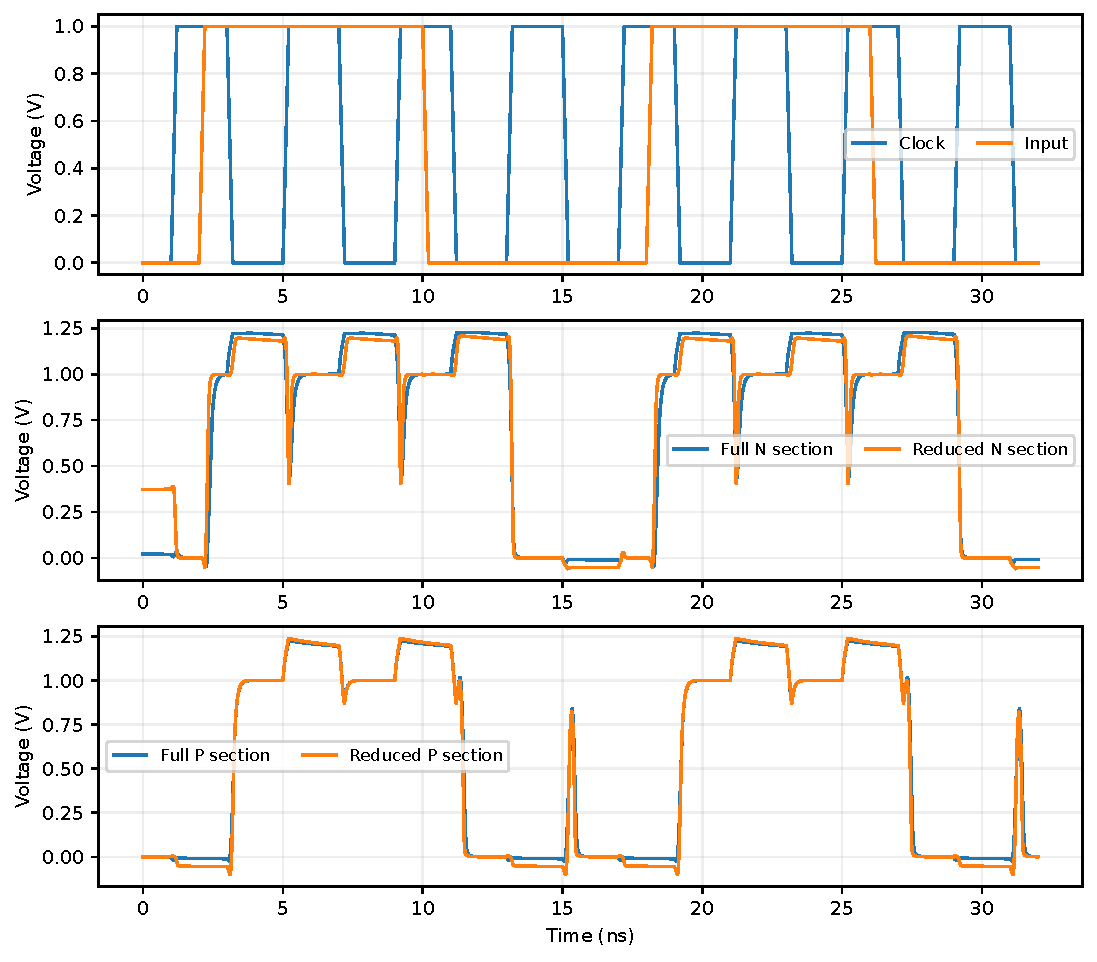
\includegraphics[width=.96\linewidth]{figures/latch_equivalence.pdf}
\caption{完整與簡化 latch 的配對；邏輯相符不代表類比波形完全一致。}
\end{figure}

6 個取樣時點的配對邏輯相同，N section 最大差 0.174150 V，P section 為 0.043550 V。部分高電位超過 1 V、低電位略低於 0 V，來自浮接節點與 clock feedthrough；這些電位不應裁切成理想 0/1 後再聲稱兩者相同。

\begin{center}
\small
\setlength{\tabcolsep}{4pt}
\begin{tabular}{lrrr}
\toprule
雙 inverter & 保持窗最小 (V) & 最大 (V) & 變動幅度 (V) \\
\midrule
n & -0.052238 & -0.038262 & 0.013977 \\
p & 1.185680 & 1.214528 & 0.028848 \\
\bottomrule
\end{tabular}
\end{center}

\begin{figure}[htbp]
\centering
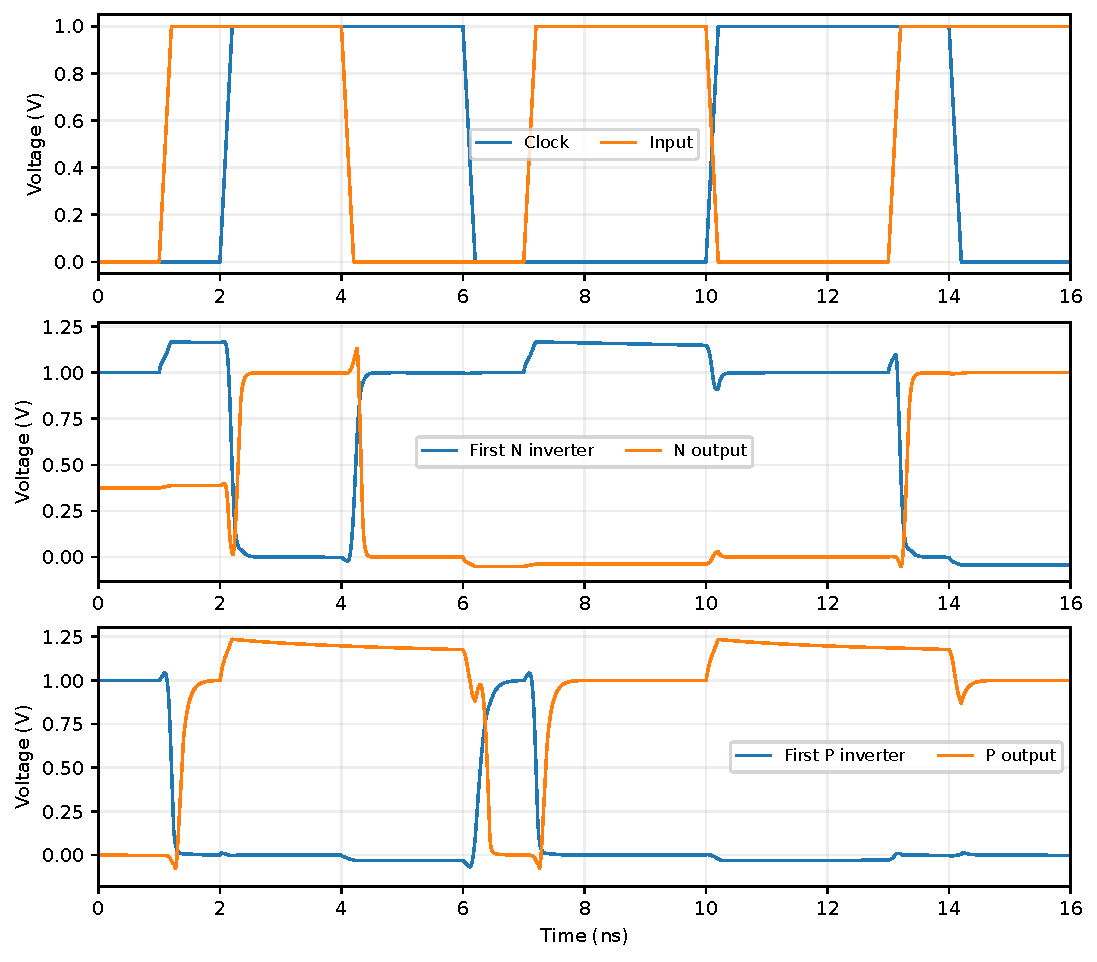
\includegraphics[width=.96\linewidth]{figures/doubled_inverters.pdf}
\caption{N 組在 7--9 ns、P 組在 3--5 ns 的保持窗內，輸入仍有變動。}
\end{figure}

N 組保持低、P 組保持高，但類比電位分別約 -0.05 V 與 1.2 V；保持邏輯正確與維持理想供應軌是兩件事。

\begin{center}
\small
\setlength{\tabcolsep}{4pt}
\begin{tabular}{lrr}
\toprule
clock edge (ns) & 輸出 & 正確樣本/6 \\
\midrule
0.2 & f1 & 6 \\
0.2 & f2 & 6 \\
0.2 & s1 & 6 \\
0.2 & s2 & 6 \\
1 & f1 & 6 \\
1 & f2 & 6 \\
1 & s1 & 6 \\
1 & s2 & 6 \\
\bottomrule
\end{tabular}
\end{center}

\begin{figure}[htbp]
\centering
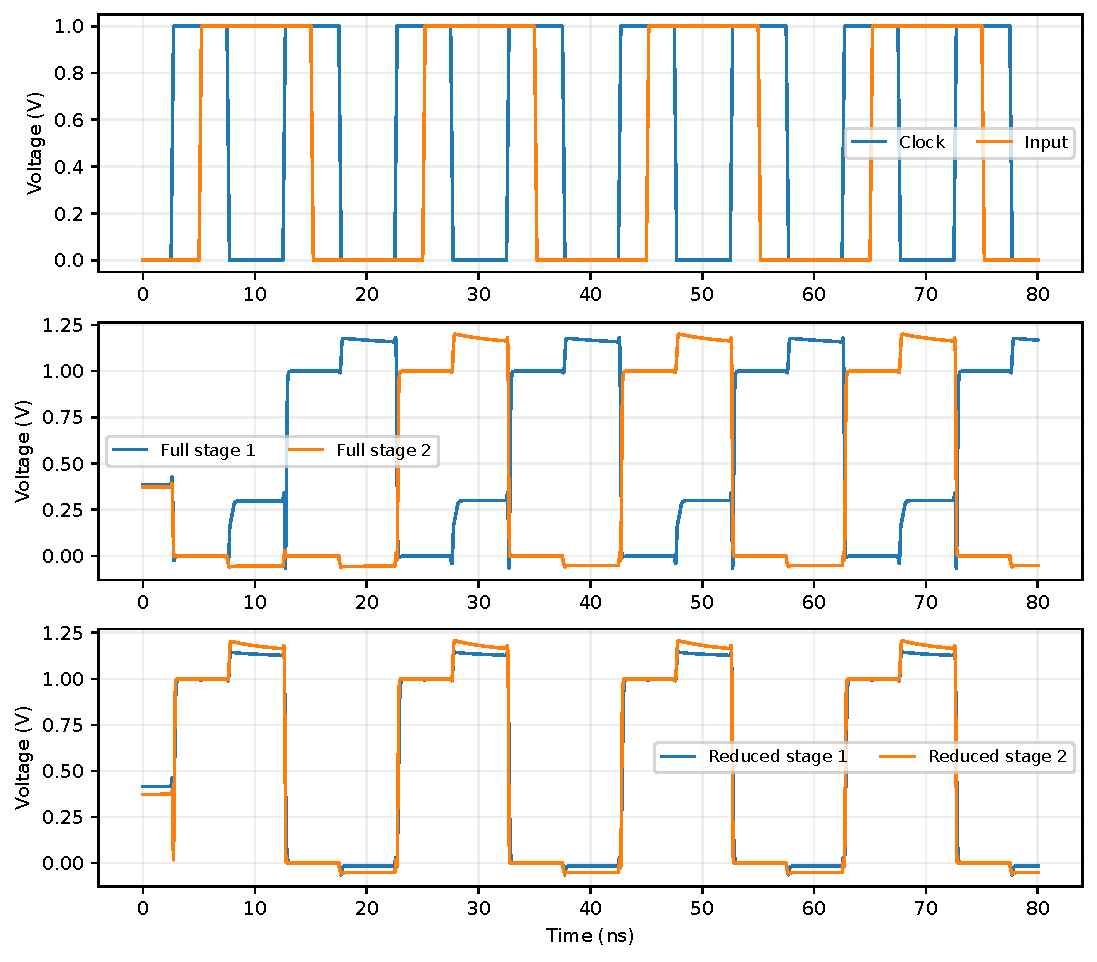
\includegraphics[width=.96\linewidth]{figures/cascade.pdf}
\caption{規律資料下的兩級完整/縮減 DFF；第一級極性不同。}
\end{figure}

0.2 ns 與 1 ns 兩種 clock edge 下，四個輸出在選定時點都得到 6/6 正確。此規律輸入在高相位中途改變並於下一個低相位開始前已建立，不能證明所有相位內資料變動皆被接受。

\subsection{限制測試與內部節點}

\begin{figure}[htbp]
\centering
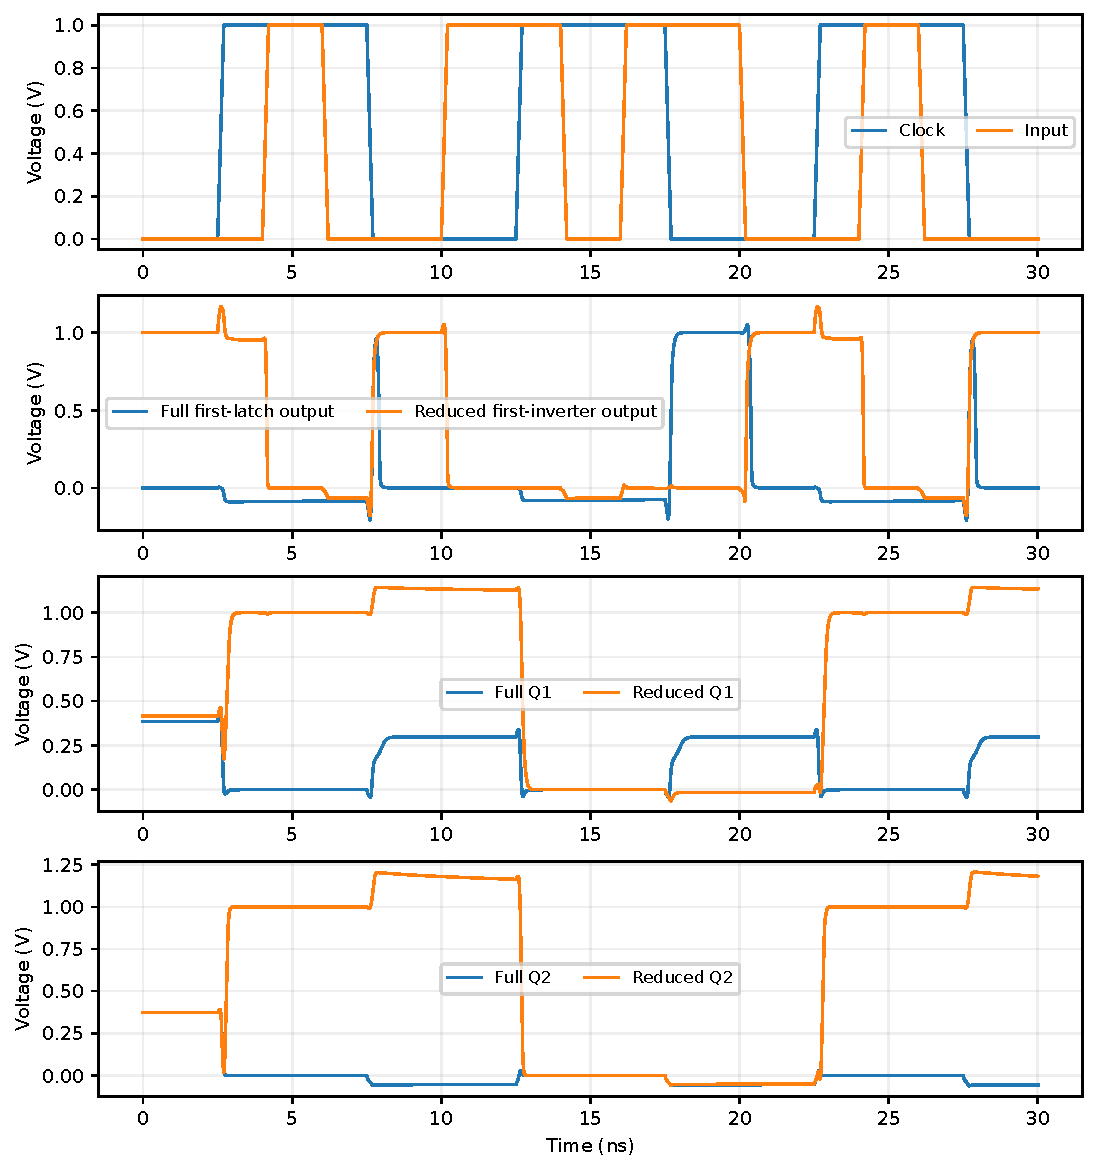
\includegraphics[width=.96\linewidth]{figures/input_timing_limit.pdf}
\caption{額外資料時序測試；完整動態 P 第一級會記住先前評估電荷，縮減版有不同的內部保持方式。}
\end{figure}

clock 於 2.5、12.5、22.5 ns 開始上升。第一次高相位中，輸入由 0 升到 1 再回 0，縮減內部節點從 0.953449 V 變為 -0.063530 V，而輸出仍約 0.999933 V，顯示內部節點不具完整靜態保持但已完成的評估可以維持輸出。完整第一個 latch 輸出同期由 -0.087237 到 -0.081927 V。

第二週期在低相位內 10 ns 才把輸入 0→1，完整 P-dynamic 第一節點先前已充高，低相位沒有把它放低的通路，因此完整第一級在 16.8 ns 仍約 0 V，未捕捉一般正緣 DFF 會預期的 1。縮減第一級當時約 0 V，符合其反相輸出；兩級鏈亦顯示不同資料序列。這是依講義拓樸保留的限制反例，不是把取樣失敗刪掉或把電路改成其他靜態 DFF。

\section{討論、差異與尚未證實的範圍}

問題 1/2 的「能否正確操作」必須附帶資料時序條件：規律測試可工作，任意相位內改資料則不具一般 DFF 的無條件等價。完整第一個 P-dynamic 級特別受單調評估限制；縮減版雖在新增測試保持預期邏輯，仍有部分浮接內部節點，需保留 setup/hold、漏電與 clock-edge 的限制。沒有將 6/6 定點結果外推成完整保持窗、所有初始條件或任意頻率保證。講義圖 28.5 中的 26.1(c/d) 標籤依上下文明確解讀為 28.1(c/d)。
